% !TeX root = ../SDonchezThesis.tex

\chapter{Decryption Core Scheduling Engine}\label{ch:edfScheduling}

Since the AES engine is decrypting a bitstream, as opposed to a simple key (as is the case in the KAC engine), it will necessarily be occupied for a considerably longer period of time than the KAC engine for each reconfiguration cycle. Furthermore, since the trend in cloud infrastructure is to implement large devices with many partitions rather than many smaller ones, it is likely that a single AES engine per PFPGA will be insufficient to accommodate the partial reconfiguration needs of said device's tenants.

To this end, this architecture proposes the implementation of multiple discrete AES cores, each of which may be attached to a partition for the purposes of facilitating a decryption operation as part of the reconfiguration process. This necessitates the scheduling and allocation of these resources in a fashion that takes into account the real-world constraints of the CSP. To this end, this architecture proposes a modified Earliest Deadline First (EDF) scheduling algorithm, to be implemented on the Hard Processor System (HPS) of the heterogenous system. This algorithm, including its assumptions, constraints, and design, is outlined in the following sections.

\section{Background}\label{sec:EDFRelated}

The concept of utilizing an EDF-based algorithm for scheduling in a real-time environment is hardly a novel idea. In fact, this application was first suggested in 1973 by Liu and Layland in \cite{liu_scheduling_1973}. In their work, the authors propose an algorithm by which independent, periodic tasks with hard deadlines and constant execution times can be efficiently scheduled prior to execution as to ensure each executes before its respective deadline. This algorithm is known as the Earliest Deadline First (EDF) scheduling algorithm. As its name suggests, the algorithm is based on the assumption that maximum utilization of a processor can be achieved by scheduling for immediate execution the task with the nearest deadline, provided that the total utilization required to execute all tasks is less than or equal to the processor's capacity.

The various qualifiers present on the word ``task'' in the above statement are critical, as they are largely incompatible with both modern programming paradigms and with the use of EDF to schedule FPGA-based tasks. In fact, the tasks executed in the use case of a CSP provisioning FPGA partitions can be generally characterized as being aperiodic, featuring flexible deadlines, and, potentially, being interdependent. Furthermore, the original EDF algorithm is a static, a priori algorithm, meaning that the task information is known in advance, and that the algorithm precomputes the optimal schedule before execution begins. The algorithm is then incapable of adapting to any modifications of the task information that may occur during the course of the execution.

In the years that have elapsed since Liu and Layland first presented the algorithm, countless modifications have been proposed which address many of these concerns. In \cite{stankovic_deadline_1998}, the application of the EDF algorithm's key principles to real-time environments (wherein the scheduler is employed dynamically at run time as opposed to a priori). Similarly, \cite{spuri_efficient_1994} enhances the EDF algorithm to accurately schedule aperiodic tasks in conjunction with periodic tasks.

A major shift in scheduling came in the early 2000s with the mass popularity of the multi-core processor. Originally the exclusive domain of supercomputers, multi-core processors became a mainstay of personal computing as a means of avoiding the immense thermal loads associated with the increasing frequency of conventional, single core CPUs. As these processors entered enterprise and consumer markets, it became clear that there was a need to efficiently distribute task load across the various cores. In \cite{abeni_edf_2020}, the authors propose modifications to the EDF algorithm to accommodate multiple cores by means of an ``adaptive migration'' algorithm that emphasizes the minimization of unnecessary task migration between cores.

One constant throughout these developments is that in most cases, the EDF algorithm and its derivatives are intended to schedule tasks on a traditional general purpose processor, whether said processor is a small microcontroller or a large multi-core AMD or Intel flagship. The application of such an algorithm to FPGAs has not previously been considered in the literature, as FPGA-based operations are typically conducted in parallel. Fortunately, most of the concepts upon which the EDF algorithm are based are also perfectly applicable to the scheduling of FPGA-based IP cores. The remaining sections of this chapter outline the application of an EDF-derivative algorithm for this use case.

\section{Assumptions}\label{subsec:EDFAssumptions}
The following assumptions are made regarding the implementation of the AES core scheduling process for this architecture:
\begin{itemize}
    \item The time required to decrypt a given partial bitstream increases linearly with a corresponding increase in file size.
    \item The time required to decrypt a given partial bitstream can be approximated into a discrete number of ``time units''.
    \item Deadlines for decryption are made available as tasks are received, and are driven by real world constraints (License Agreements, Pricing Tier, etc.).
    \item The CSP will not allocate more decryption jobs to the PFPGA than can be scheduled within their given deadlines (meaning that the schedulability does not need to be verified).
    \item The time required to switch from processing one bitstream to processing another is both non-trivial and constant.
    \item The act of reading (ingesting) and writing (outputting) bitstream segments to/from the AES engine requires a known, constant time.
    \item The time required for communication between the HPS and the AES core is assumed to be both constant and trivial.
    \item Due to the nature of the environment in which the algorithm is being implemented, it is important to note that tasks are random and likely aperiodic in nature.
\end{itemize}

\section{Constraints}\label{subsec:EDFConstraints}
The implementation outlined in subsequent sections will be subject to the following set of design constraints, imposed by the assumptions listed in the preceding section as well as best practices:
\begin{itemize}
    \item In the event of a tie between two task for the next time unit, where one task is the task that was operated on in the previous time unit, the task which was previously being executed shall continue to be executed, in order to eliminate overhead associated with context switching between tasks.
    \item As the IP core currently selected for performing the AES decryption operation is non-pipelined, and therefore not capable of transitioning seamlessly between decryption operations without first having its state machine reset, there shall be a small reset delay during context switches
    \item The algorithm shall be implemented for an abstract number of AES cores N, with the assumption that N shall be some small number in the real-world implementation.
    \item The HPS shall communicate with the AES cores via the AXI bus.
    \item The bitstream shall reside in the domain of the PS for purposes of this algorithm, and shall be transferred via the AXI bus.
    \item The atomic unit of the bitstream shall be considered sufficiently large, as too small of an atomic unit will cause scheduling computations to take longer than the time unit itself.
    \item Tasks are placed in a queue, Q, arranged by deadline in ascending order (such that the earliest deadline is at the start of the queue). 
    \item The deadline associated with a processor is the deadline of the task it is currently executing, or $\infty$ if it is idle.
\end{itemize}

\section{Proposed Scheduling Algorithm}\label{subsec:AlgoImpl}
Algorithm \ref{alg:EDFAES} implements the scheduling routine for the AES Cores, as governed by the constraints and assumptions outlined above. This algorithm serves as the guidance for the implementation of the Scheduler as outlined in subsequent sections, subject to the constraints and assumptions outlined above.
\begin{algorithm}
    \caption{Global EDF Scheduling Algorithm for AES Decryption Cores}\label{alg:EDFAES}
    \begin{algorithmic}

        %define foreach since it isn't included
        % \algnewcommand\algorithmicforeach{\textbf{for each}}
        % \algdef{S}[FOR]{ForEach}[1]{\algorithmicforeach\ #1\ \algorithmicdo}
        % \algnewcommand\algorithmicendforeach{\textbf{end for each}}
        % \algdef{E}[FOR]{EndForEach}[1]{\algorithmicendforeach\ #1\ \algorithmicend}
        \State We consider a task set $\uptau$ consisting of $x$ tasks $T_1$ , . . . , $T_n$ that are sporadically released from the CSP with arbitrary deadlines
        \State Variables: 
        \State N - the set of cores to be utilized
        \State Q - the queue containing all tasks currently pending execution
        \State $T_{n_i}$ - the task assigned to a given core
        \State $D_t$ - the delay associated with a given task
        \State $D_{n_i}$ - the delay associated with the task currently executing on a core (for brevity)
        \State $D_{Q_i}$ - the delay associated with the task at a given position in the queue (for brevity)

        \\

        \Require $n(N) > 0$ \Comment{There are a nonzero number of cores}

        \Function{SwapTaskToQueue}{$T$}
            \ForAll {$Q_i \in Q$} 
                \If{$D_T < D_{Q_I}$}
                    \State Insert $T$ into $Q$ at index $Q_i$
                    \State \Return pop($Q$)
                \EndIf
            \EndFor
            \State Append $T$ to the end of $Q$ \Comment{If all currently queued tasks expire before $T$}
        \EndFunction

        \\

        \While{true} \Comment{Each Time Unit}
            \ForAll {$n_i \in N $}
                \If{$Q \neq \emptyset$}
                    \If{$D_{n_i} == \infty$}
                        \State $T_{n_i} \gets T_{Q_0}$ \Comment{Pop $Q$}

                    \\
                    \State \Comment {\parbox[t]{.75\linewidth}{If the currently executing task has a later deadline than the first task in the queue and has the latest deadline of any currently executing task across all cores.}}
                    \\

                    \ElsIf{$(D_{n_i} > D_{Q_0})$ AND $D_{n_i} == max(D_N)$}  
                        \State $T_{n_i} \gets $SwapTaskToQueue($T_{n_i}$)
                    \Else
                        \State $T_{n_i} \gets T_{n_i}$
                    \EndIf
                \EndIf
            \EndFor
        \EndWhile
    \end{algorithmic}
\end{algorithm}

It should be noted that, by virtue of comparing the deadline of the first task in the queue against the latest deadline of all currently executing tasks, this algorithm supports preemption. Such a consideration is critical for the success of a scheduler dealing with tasks of varied size, as otherwise a large but long-lead task could cause a short, more urgent task to miss its deadline when both could have been scheduled effectively.

\subsection{Task Model}\label{subsec:TaskModel}
The algorithm outlined in Algorithm \ref{alg:EDFAES} centers around the notion of a task, which is representative of a tenant bitstream that is to be decrypted. From the perspective of the scheduler itself, the task does not necessarily contain this bitstream, as the scheduler is not concerned with the contents of the PL. Rather, the scheduler is provided only with metadata about the task, such as is necessary to schedule it for execution. The following information is stored in this task model:

\begin{itemize}
    \item A Unique ID (arbitrarily constructed) used to refer to the task
    \item A ``human-readable'' name for the task
    \item The number of discrete Time Units of execution the task requires for decryption
    \item The task's deadline
    \item The period of the task, represented as zero if the task is aperiodic
\end{itemize}
In the implementation described below, this information is contained in a JSON structure. Other encoding schemes are certainly feasible, and the software as implemented also supports XML formats when compiled appropriately. An example of a task model is given in the listing below.

\begin{lstlisting}[language=json, caption={An example task object, presented in JSON}, captionpos=b, float]
{
    "deadline": 15,
    "unitsToExecute": 5,
    "taskId": 1,
    "taskName": "Task 1",
    "period": 20
}
\end{lstlisting}

\section{Algorithm Implementation}\label{sec:Impl}

This effort implemented the above algorithm in a test application which is representative of its implementation in the real-world use case outlined in Chapter \ref{ch:systemArchitecture}. However, as the scope of the research completed to date does not include the larger system outlined in that section, it is somewhat constrained with regards to its external interfaces. Namely, it does not attempt to directly affect any actual IP Cores, but rather performs theoretical scheduling of the cores and notes its results in a log file. It does, however, attempt to mimic the likely real-world method of input, in that it parses serialized data such as would be suitable for transmission by a discrete centralized controller overseeing a number of PFPGA instances.

Along with the development of the Scheduler itself, it was also necessary to thoroughly exercise the application to ensure that it functions successfully under load. As a result, it was also necessary to develop a Testbench application, which is capable of generating arbitrary tasks for the AES cores to schedule. This Testbench is capable of generating tasks in accordance with a given target utilization rate. A comprehensive set of Inter-Process Communication (IPC) calls enable synchronization between the two applications. For purposes of ensuring low resource utilization, as well as promoting well organized source code, both of these applications were developed in C++, utilizing an object-oriented approach. Section \ref{subsec:SchedulerImpl}, below, outlines the implementation of the Scheduler itself, while Section \ref{subsec:TestbenchImpl} outlines the implementation of the Testbench. Section \ref{subsec:IPC} outlines the interconnection of these two applications.

\subsection{Scheduler Implementation}\label{subsec:SchedulerImpl}
The Scheduler application consists of several interrelated threads operating in parallel. First among these is an input parser, which waits for serialized task information and, upon receipt, deserializes it into task objects. For the sake of best practices (as well as ease of parsing), this data is encapsulated in a JavaScript Object Notation (JSON) string, which, despite its name, is a language agnostic structure that is commonly used to represent entities. In its current implementation this data is simply read from a file descriptor (such as standard input), although future extensibility to a socket based architecture for network communications is possible.

Alongside the input parser is the timer manager. The timer manager is responsible for managing the discrete units of time for which the cores can be scheduled. The AES cores intended for use in the larger research effort are currently non-pipelined cores requiring a fixed number of clock cycles to process each word of data. Accordingly, the frequency with which they can be scheduled is based on a multiple of that number of clock cycles, which must be small enough to afford flexibility but high enough to minimize wasted cost due to context switching (per the design assumptions). As the HPS and the PL do not necessarily share a common clock, and as the execution of the various threads on the processor is non-deterministic in its own scheduling, it is necessary to utilize a timer to ensure scheduling operations are executed exactly once per atomic unit of IP Core schedulability. This thread provides that functionality, and sets flags for the other threads as needed to facilitate their operation.

The final (and arguably most consequential) thread of the Scheduler application is the core servicer itself, which is responsible for ensuring each core is executing the ideal task per the prescribed algorithm. Once per Time Unit, the core servicer evaluates the deadlines of the tasks currently executing on the cores against those contained in the Scheduler's Task Queue, and performs substitutions as necessary to ensure that the tasks with the nearest deadlines are those currently in execution. 

For purposes of this effort, these services are implemented using C++'s standard threading library (as opposed to the more traditional ``pthread'' library). This threading implementation was chosen to promote cross-platform interoperability, as well as performance optimization where possible.


\subsection{Testbench Implementation}\label{subsec:TestbenchImpl}
The Testbench application in in many ways appreciably simpler than the Scheduler itself. It is only a single threaded application, and the task it performs is straightforward - it simply creates tasks populated with arbitrary information. However, this seemingly straightforward operation is greatly complicated by one of the assumptions outlined in Section \ref{subsec:EDFAssumptions} above. Namely it is the fourth assumption in that section which proves problematic: The CSP will not allocate more decryption jobs to the PFPGA than can be scheduled within their given deadlines. This greatly eased the development of the Scheduler itself, by eliminating the need for it to perform schedulability checks as part of its task processing. However, as the Testbench is effectively serving as the CSP in these simulations, it falls to the Testbench to ensure that the tasks it generates do not overload the PFPGA instance for which the Scheduler is allocating resources.

This is accomplished through introducing some element of reporting to the Scheduler itself, and making those results available to the Testbench. Specifically, the Scheduler maintains a table outlining how many outstanding time units need to be executed by any given point in time, as described by the sum of all of the outstanding units for each task due at that point. By combining this information with knowledge of what unit in time the PFPGA and PS are currently in, it is possible to validate in real time the schedulability of a task as it is being generated, and to make adjustments as needed. 

This logic is captured in Equation \ref{equ:Utilization}, below. In this equation, $t_c$ represents the current Time Unit, $t_n$ represents the time unit being proposed as the deadline for the task, $D_i$ represents the number of units due at time $i$, and $UtE$ represents the number of Units to Execute for the task currently being evaluated. $P$ is the parallelization factor, or the number of cores which the schedule is being distributed between, while $n-c$ yields the total number of TimeUnits between the time the equation is evaluated and when the deadline will come. The ``Desired Load Percentage'' is the target utilization rate for the cores.

\begin{equation}\label{equ:Utilization}
    \frac{(\sum_{i=t_c}^{t_n}D_i)+UtE}{P*(n-c)} < Desired\:Load\:Percentage
\end{equation}

By verifying the validity of this equation for each generated task's proposed deadline, it is possible to ensure that target average utilization is not exceeded. Furthermore, the maintenance of this information on the part of the Scheduler is non-resource intensive, requiring a single addition operation as each task is parsed, a single decrement operation as each core is serviced, and a single increment operation (for the current unit counter) on the part of timer manager per Time Unit.

Unfortunately, this does not fully resolve the issue outlined above. In addition to ensuring that the average utilization is not compromised, it is also important to verify that the instantaneous utilization never exceeds the maximum. (For example, inserting a task that has a Units to Execute value of 100 with a deadline of 500 may not compromise the average utilization, but may cause a task due at unit 510 to lack sufficient time to run). To rectify this, an additional check is necessary. 

To perform this additional check, the generator iterates across the entire simulation window, computing a running sum of the outstanding work to be done that is due at that unit, and comparing that value plus a prorated portion of the new task's units against the theoretical limit. This check is captured by Equation \ref{equ:InstUtil}:
\begin{equation}\label{equ:InstUtil}
    \sum_{i=t_0}^{t_n}D_i + \max(\min(UtE, i - t_c), 0) < P*(n-i-c)\:\forall i>c
\end{equation}

Provided the conditions of both Equations \ref{equ:Utilization} and \ref{equ:InstUtil}, above, are satisfied, the Testbench application can then assume that the proposed deadline is valid for the generated task.

\subsection{Inter-Process Communications}\label{subsec:IPC}
The inclusion of an operating system into this research effort greatly eased efforts to facilitate communication between the two discrete applications. Both Windows and Linux implement comprehensive facilities for Inter-Process Communication (IPC), which enable the transfer of data between applications. Unfortunately, the two systems do not have a common set of IPC functions, requiring slightly difference implementations to satisfy the two architectures. Despite this, the overall design of the IPC structures for the two architectures is effectively the same.

\subsubsection{Testbench to Scheduler Communication}\label{subsubsec:TestbenchSchedIPC}
Communication from the Testbench application to the Scheduler application is straightforward, as the only traffic flowing in this direction is the serialized task data. Since this data is serialized and relatively small in size, and in the interest of replicating the real-world functionality of the software, this data is simply read in from a file descriptor. In Windows, this is accomplished via a Named Pipe, which effectively enables the data to be consumed as if it were typed into the standard input of the application in the terminal window in which it is executing. Specifically, this named pipe was configured in ``message'' mode, such that the entire task is treated as an atomic unit for purposes of the transfer, rather than its constituent bytes (the latter configuration can result in multiple or even partial messages being sent as a single input, which would unnecessarily complicate the parsing operation).

Linux also provides a ``Named Pipe'' functionality, but this functionality is strictly byte-oriented as opposed to message-based. Accordingly, it is not desirable for use in this scenario. Fortunately, the Linux system also supports System-V Message Queues, a part of the POSIX standard that is functionally equivalent to Windows's Named Pipes in message mode. The only impactful difference between the Windows and Linux implementations of this facility is that the Linux implementation does not facilitate the ability to wait for a connection, thus requiring the use of a Semaphore (another POSIX IPC method) to ensure synchronization between the two applications.

\subsubsection{Scheduler to Testbench Communication}\label{subsubsec:SchedTestbenchIPC}
The transfer of data from the Scheduler to the Testbench is appreciably more complex, as the table of Outstanding Units Due (used in Equation \ref{equ:Utilization}) is updated during each TimeUnit, and contains $P*N$ words of data, where N is the number of time units to simulate and P is the number of IP Cores. It would be inefficient to the point of impracticability to transfer and parse that data every time unit, as its scale for even modest simulations would likely consume a non-trivial portion of the available compute time to parse. Accordingly, the implementation instead uses a shared memory space for the purposes of facilitating this communication, accomplished in Windows by utilizing the File Mapping functionality of the Win32 API, and in Linux via the comparable Shared Memory Segment functionality. In this way, the generator simply receives a pointer to the Scheduler's own copy of the table, and is always able to view the latest updates to it without any need for direct transfer between the applications.

The same functionality is utilized for the mapping of the current Time Unit between the two systems, as it eliminates any edge cases wherein the unit changes shortly after the Testbench queries it. This allows for the most accurate possible scheduling of tasks.

\section{Development and Test Environment}\label{sec:environment}
The implementation above utilized a number of development tools and platforms, and targets a specific set of hardware and supporting software as outlined in the following subsections. While it may (and likely will) execute under other conditions, the performance of the algorithm cannot be guaranteed outside of the specified test environment.

\subsection{Target Hardware}\label{subsec:targetHW}
The Scheduler and testbench implemented in \ref{sec:Impl} target the AVNet ZedBoard Development Board. The ZedBoard contains a Xilinx XC7Z020-CLG484-1 heterogenous SoC, featuring a Dual-Core AR Cortex-A9 MPCore processor and an Artix-7 series FPGA with 85,000 logic cells. The board also features 512MB of DDR3 memory, 256Mb of QuadSPI Flash memory, and a 10/100/1000 Ethernet Interface. It also has integrated JTAG and PS UART interfaces, which greatly simplifies the loading and debugging of the applications and bitstreams used in the testing process. A diagram of the ZedBoard, with key I/O connections indicated, is provided in Figure \ref{fig:zedImg}.

\begin{figure}[ht]
    \centering
    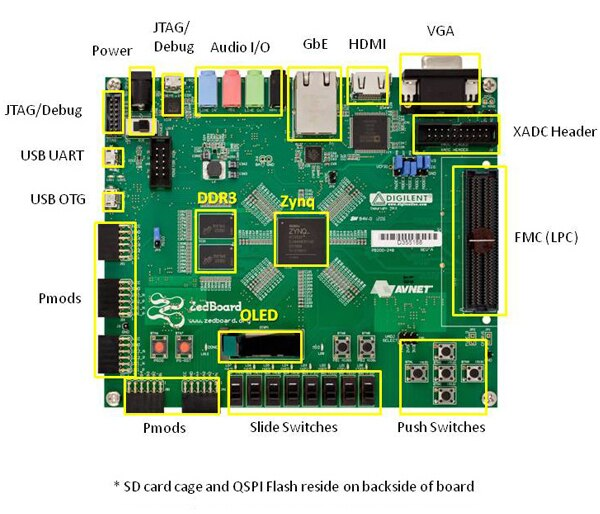
\includegraphics[width=0.8\textwidth]{ZedBoard-Overlay.jpg}
    \caption[ZedBoard Schematic]{ZedBoard Schematic, with key I/O \cite{noauthor_zedboard_nodate}.}
    \label{fig:zedImg}
\end{figure}

For purposes of evaluating the performance of the scheduler implementation, the PL of the ZedBoard was loaded with AVNet's stock reference design, which instantiates the PS-PL interfaces, the DDR3 controller, and the various General Purpose Input Output (GPIO) modules. This design is depicted in Figure \ref{fig:zedGPIODesign}. More robust implementation of the scheduler such as would be suited for full integration into the architecture developed in Chapter \ref{ch:systemArchitecture} would require the use of a customized design. Figure \ref{fig:zedResourceConsumption} provides statistical data demonstrating the resource utilization associated with this design. As is clear from the data, the ZedBoard's resources are more than ample for this simple design, despite its age. That being said, the implementation of multiple AES (and KAC) cores would likely tax its resources such that it would be unsuitable for use. Consequently, further research efforts seeking to fully implement the entire architecture proposed in Chapter \ref{ch:systemArchitecture} would likely need a more modern, larger FPGA.

\begin{figure}
    \centering
    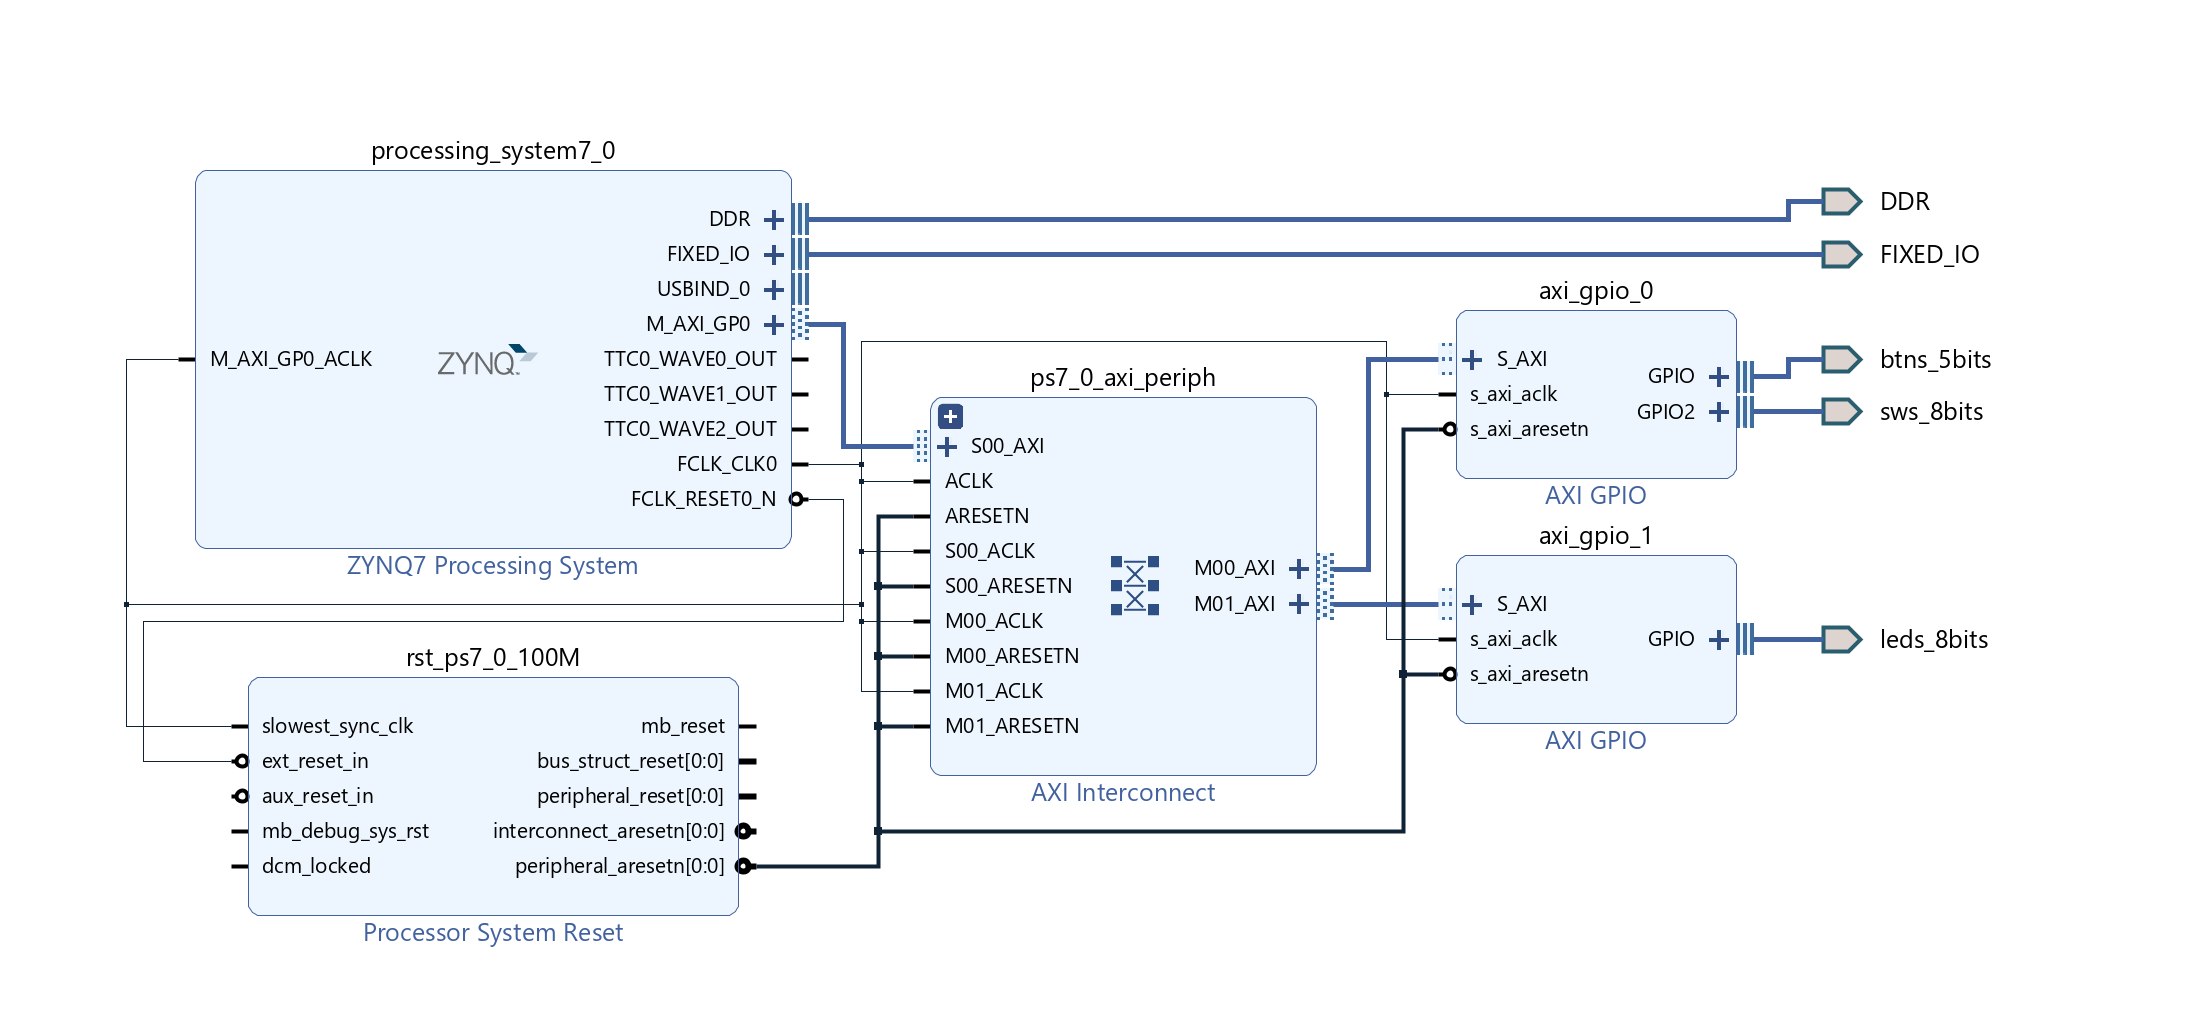
\includegraphics[width=0.8\textwidth]{zed_hw_gpio_bd.png}
    \caption[ZedBoard Reference Design]{Block Diagram of the ZedBoard Reference Design}
    \label{fig:zedGPIODesign}
\end{figure}

%TODO: Add screenshot of PS Interface config - indicate that there is work involved

\begin{figure}
    \centering
    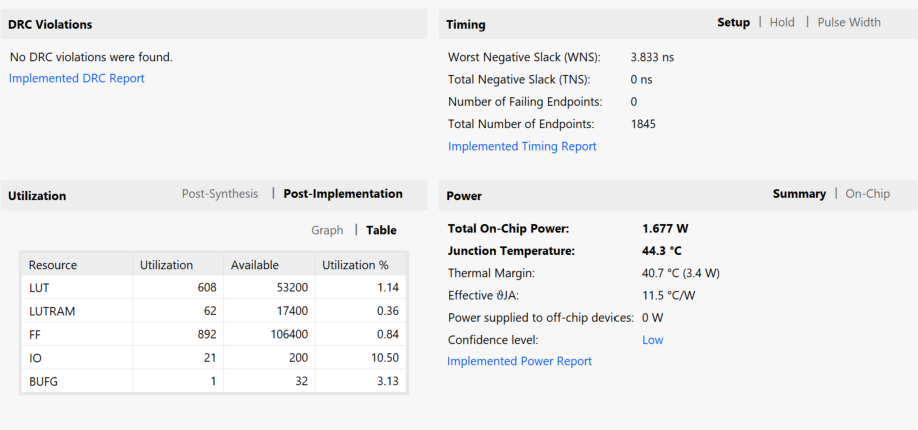
\includegraphics[width=0.8\textwidth]{zed_hw_gpio_stats.png}
    \caption[ZedBoard Resource Consumption]{ZedBoard Resource Consumption}
    \label{fig:zedResourceConsumption}
\end{figure}

\subsection{Target Operating System}\label{subsec:os}
By virtue of introducing multiple threads to the scheduler (and also by virtue of running two applications on a single core processor), it is necessary to implement an operating system (OS) on the processor system upon which the scheduler simulation is running. Furthermore, the larger design will add additional functionality to the processor system, further necessitating an operating system for thread management and for scheduling of the processor itself. To this end, several operating system choices were considered for implementation on the hardware target in support of this simulation. As the target in question includes a Xilinx SoC, it was decided that the ideal choice for such a system would be the Xilinx PetaLinux OS, as it includes all of the necessary drivers for interfacing with the various devices on the development platform. Additionally, the PetaLinux platform is based on the OpenEmbedded Project's toolchain, which affords tremendous flexibility and customization potential as needed. For purposes of this effort, PetaLinux 2020.2 was chosen for compatibility with the equivalent versions of the Xilinx design tools (discussed in Subsection \ref{subsec:devEnv}, below) already in use. This PetaLinux version is derived from Linux kernel version 5.4.

For ease of development and testing, the two software applications were designed to run both in the native Windows environment of the development computer as well as the Linux environment of the target. This reduced cycle time between incremental iterations of the applications, as well as eliminated dependence on an extensive physical setup for testing.

\subsection{Development Environment}\label{subsec:devEnv}
Although the hardware specifications of a development machine are of little consequence to the implementation itself, they are provided here for sake of completeness and perspective to those attempting to replicate the results. The development machine used by the authors in the course of this project was a Windows 10 Professional Edition 64-bit laptop featuring an Intel Core i7-9750H CPU with a base frequency of 2.60GHz. The machine featured 16 GB of DDR4 DRAM and a 1 TB SSD.

The scheduler and testbench applications were first developed for Windows to ease testing, and then later ported to the hardware target. For Windows development, the author utilized Visual Studio 2019 Enterprise Edition, which is available to students free of charge through Microsoft's Azure for Students program. It should be noted, however, that the enhanced feature set of the enterprise edition was not strictly necessary, and that implementation and compilation using the community edition (which is free of charge to all users) is certainly possible.

The construction of the PetaLinux operating environment outlined in \ref{subsec:os} requires a Linux environment. To this end, the author constructed a Docker container based on the ubuntu:18.04 image, and extended with the full Xilinx 2020.2 toolchain (Vivado, Vitis, and the PetaLinux toolchain). The container was used for all stages of the Linux port and implementation, from hardware export to operating system implementation to application compilation. The container was wrapped in a Visual Studio Code devcontainer, a Microsoft concept that automates the construction of docker images and integrates them into the Visual Studio Code ecosystem, for sake of convenience. Note that users will need to provide their own Xilinx installers and license files.

\section{Experimental Results and Discussion}\label{sec:findings}
The implementation of the EDF algorithm and Testbench on the Windows target has revealed that it is able to successfully schedule tasks at high utilization levels with low miss rates, given that the requirements outlined in the design constraints and assumptions are met. Careful analysis of the Scheduler's output reveals that it is scheduling in accordance with the algorithm, with only a single exception - at the end of the simulation, as the task queue depletes, the Scheduler unnecessarily shifts tasks from higher index cores to vacant lower-indexed cores. Ultimately, this inconsistency is non-consequential, as in a real-world implementation it is unlikely that the task queue would ever be depleted (and also as it does not cause any tasks to miss their deadline).

\subsection{Scheduler Effectiveness at Varying Utilization Levels}\label{subsec:SchedulerDataUtilVary}
As the primary measure of success for this Scheduler implementation is how it performs under heavy load, a series of trials were conducted on the hardware target under varying levels of load in order to determine the average performance of the algorithm for each loading. These results are described in Table \ref{table:SchedEffectivenessUtilVary}, below. All iterations were performed for a simulation of 1000 TimeUnits, with the number of decryption cores fixed at 4. The results below are computed from the average of three trials for each utilization, each utilizing a different randomly generated set of tasks.

\begin{table}[ht!]
    \centering\begin{tabular}{| c | c | c | c |}
        \hline
        Target Utilization & Number of Tasks & Units Elapsed & \% Units Missed \\
        \hline
        50\% & 38 & 512 & 0\% \\
        60\% & 47 & 604 & 0\% \\
        70\% & 53 & 732 & 0\% \\
        80\% & 64 & 825 & 0\% \\
        90\% & 74 & 925 & 0.15\% \\
        100\% & 82 & 1000 & 8.63\% \\
        \hline
    \end{tabular}
    \caption{Scheduler effectiveness at varying utilization with fixed core count}
    \label{table:SchedEffectivenessUtilVary}
\end{table}

These findings indicate a high level of success on the part of the scheduling algorithm, as it effectively schedules tasks even at high levels of utilization. It is worth noting that the case of 100\% utilization is a special case, as a detailed analysis of individual runs reveals some discrepancies that explain the high miss rate. The current implementation of the Testbench does not immediately send a task at TimeUnit = 0 on every iteration, as its operation is, by design, random. As a result, the logged allocation of cores to tasks often indicates empty cores for the first several TimeUnits. However, the Testbench is still attempting to generate 100\% of the TimeUnits (4000 in the case of these trials), meaning that it will occasionally overschedule the processor. It has been observed through additional experimentation that the increase in miss rate between 90\% and 100\% utilization more nearly approximates an exponential line of best fit than a linear one, further validating the performance of the algorithm.

\subsection{Performance Evaluation at Varying Utilization Levels}\label{subsec:performanceDataUtilVary}
Although the effectiveness of the algorithm (and its implementation) are by far the most important criteria for evaluating their success, it is also important to consider the performance of the application. In the context of the larger system outlined in Chapter \ref{ch:systemArchitecture}, a number of other processes will likely have to execute on the single core available on the hardware target. Accordingly, it is crucial that the Scheduler is not overtaxing the HPS, such that the other portions of the system are also able to execute as needed. Accordingly, Table \ref{table:SchedPerfUtilVary}, below, reports on the total utilization time of the processor for each of the iterations above.

\begin{table}[ht!]
    \centering\begin{tabular}{| c | c | c | c | c |}
        \hline
        Utilization & Clock Time & User Time & System Time & RAM Used \\
        \hline
        50\% & 10.79s & 10.34s & 0.07s & 10.48MB \\
        60\% & 11.04s & 10.35s & 0.06s & 10.63MB \\
        70\% & 10.85s & 10.35s & 0.07s & 10.61MB \\
        80\% & 10.93s & 10.33s & 0.11s & 10.54MB \\
        90\% & 10.87s & 10.39s & 0.05s & 10.73MB \\
        100\% & 10.92s & 10.39s & 0.09s & 10.63MB \\
        \hline
    \end{tabular}
    \caption{Scheduler performance at varying utilization with fixed core count}
    \label{table:SchedPerfUtilVary}
\end{table}

As is evidenced in the table, Resource consumption is not closely correlated with target utilization, but appears roughly constant across all target utilization levels. This is highly beneficial in this scenario, as, with the larger and more complex Task data that will necessarily accompany real tasks being implemented on real IP, any utilization correlated growth in resource consumption would be greatly magnified (and as it is desirable to maximize utilization for revenue purposes on the part of the service provider). 

It should also be noted that much of the ``User Time'' listed in Table \ref{table:SchedPerfUtilVary} above is currently ``idle'' time. As the current implementation of the Scheduler is not controlling real IP, most of the time in each TimeUnit is spent waiting for the unit to expire. This waiting process is not optimized to minimize processor consumption in the implementation used to generate these results, as it is a placeholder for future work.

\subsection{Scheduler Effectiveness at Varying Core Counts}\label{subsec:SchedulerDataCoresVary}
In addition to understanding how the scheduler behaves under varying utilization levels, it is also critical to ensure that it works across a range of core counts. Accordingly, the scheduler was exercised at a fixed load percentage (75\%) for several trials at core counts ranging from 1 to 5 in order to further characterize the performance of the algorithm. These results are captured in Table \ref{table:SchedEffectivenessCoresVary}, below.

\begin{table}[ht!]
    \centering\begin{tabular}{| c | c | c | c |}
        \hline
        Number of Cores & Number of Tasks & Units Elapsed & \% Units Missed \\
        \hline
        1 & 15.33 & 719.67 & 0.00\% \\
        2 & 29.00 & 737.00 & 0.00\% \\
        3 & 43.67 & 774.00 & 0.55\% \\
        4 & 59.33 & 777.67 & 0.12\% \\
        5 & 79.33 & 778.00 & 0.00\% \\
        \hline
    \end{tabular}
    \caption{Scheduler effectiveness at varying core count with fixed utilization}
    \label{table:SchedEffectivenessCoresVary}
\end{table}

As can be seen here, an increase in the number of cores causes the testbench to output a proportionally larger number of tasks, although the correlation is not precise due to variations in task length (as the testbench is attempting to meet a target number of TimeUnits, not a specific task count). Furthermore, there does not appear to be a strong correlation between the number of cores and the miss rate of the scheduler, which is an critical indicator of scalability. Were there to be positive correlation, it would indicate that CSPs may have difficulty implementing such a scheme on the larger PLs that would be preferable to operate in a datacenter, as these would require a higher number of cores to service their various partitions.

\subsection{Performance Evaluation at Varying Core Counts}\label{subsec:performanceDataCoresVary}
As with the case of varying utilization levels, it is important to consider scheduler performance from a resource utilization perspective alongside one of pure accuracy, as an accurate scheduler is of limited use if it does not enable the processing system to perform the various other activities required to operate the heterogenous system. The performance characteristics of the implementation against designs with varying numbers of cores is captured in Table \ref{table:SchedPerfCoresVary}, below.

\begin{table}[ht!]
    \centering\begin{tabular}{| c | c | c | c | c |}
        \hline
        Number of Cores & Clock Time & User Time & System Time & RAM Used \\
        \hline
        1 & 11.96s & 10.31s & 0.06s & 10.74MB \\
        2 & 11.14s & 10.35s & 0.05s & 10.67MB \\
        3 & 11.04s & 10.32s & 0.10s & 10.64MB \\
        4 & 10.88s & 10.35s & 0.08s & 10.76MB \\
        5 & 11.12s & 10.38s & 0.06s & 10.67MB \\
        \hline
    \end{tabular}
    \caption{Scheduler performance at varying core count with fixed utilization}
    \label{table:SchedPerfCoresVary}
\end{table}

These results bear remarkable similarity to those discussed in Section \ref{subsec:performanceDataUtilVary}, as evidenced by the lack of correlation between the number of cores and the resource utilization. Although lack of correlation itself is not a positive, lack or correlation in conjunction with low data volatility is indicative of a constant and predictable performance, which is critical for many of the same reasons discussed in Section \ref{subsec:SchedulerDataUtilVary} pertaining to the desire of CSPs to utilize large FPGAs with many partitions and therefore multiple decryption cores.